\chapter{\label{chap:evaluation}Evaluation}
We evaluated the viability of our DAO as a Big Tech alternative. An ideal evaluation would be by measuring the impact of a large-scale (millions of users) and long term deployment of MusicDAO in terms of artist income and artist happiness. However, the time and scale required is not feasible in the scope of this thesis. Instead, we deploy MusicDAO on a smaller scale. Our system was installed and executed on 50+ Android devices in a public release. We measure performance of money transaction flow, music streaming and search latency in controlled and uncontrolled experiments. These measurements determine the responsiveness of our infrastructure in small network sizes. By comparing latency and throughput in several network sizes, we can make conclusions of the performance of our infrastructure in larger networks.

The crash-free rate of MusicDAO, throughout this public experiment, was $>94\%$ as measured by Crashlytics\footnote{\url{https://firebase.google.com/docs/crashlytics}} (see fig. \ref{fig:crash-free-users}). 

\begin{figure}
    \centering
    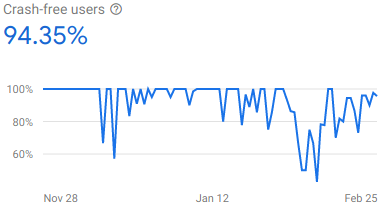
\includegraphics[width=0.4\linewidth]{evaluation/crash-free-users-90-days.png}
    \caption{Crash-free users over time, as measured by Firebase Crashlytics}
    \label{fig:crash-free-users}
\end{figure}
In a public release experiment, the MusicDAO application is published to a public audience. The test subjects are given the MusicDAO application and are asked to stream music and send money to artists, but with no specific rules or guidelines. This is an uncontrolled experiment: there is no control over the actions of the test subjects. We observe the flow of money on the Bitcoin blockchain, with a \textit{block creation interval} of 1 hour. 

In multiple \textit{controlled} experiments, we use 10 Android devices that are under our control. we measure latency and throughput of music data and money transfers, and analyze the impact of network size on these measurements.

% Discuss influence of BEP42 in bittorrent DHT network, our seedbox nodes may be blacklisted or throtled by other DHT nodes because our seedboxes are seeding a large amount of torrents (100) while having only 1 static ipv4 address

\section{Uncontrolled experiment: Public release}
MusicDAO is released publicly on the Google Play store. For the public release, 50 Creative Commons albums are used as test data (obtained from Jamendo\footnote{\url{https://www.jamendo.com/}}), for the test subjects to discover. Creation of new music releases is disabled, in order to prevent illegal content on a public network. Using datasets from Google Play, Firebase Analytics\footnote{\url{https://console.firebase.google.com}} and our Bitcoin blockchain test environment, we evaluate (1) the responsiveness of our Bitcoin faucet, (2) the block creation interval and (3) the flow of money to artists. 

\subsection{Automated starter money transactions}
\label{chap:starter-money-flow}
Upon installation and first running MusicDAO, it sends a request in the background to our Bitcoin node, asking for 10 coins in starter money. We analyze the responsiveness of this node by obtaining two datasets, and inspecting their correlation in terms of timing of events. The two datasets are: 
\begin{enumerate}
    \item App activations per day, as measured by Firebase Analytics\footnote{\url{https://console.firebase.google.com}} (\textit{first\_open} event\footnote{\url{https://support.google.com/firebase/answer/9234069?hl=en}}).
    \item Outgoing transactions from our Bitcoin node with a value of 10 coins, scraped from our blockchain.
\end{enumerate}

\textit{App activations} mean that the TrustChain Superapp is opened for the first time. This happens when (1) locally testing the app, when (2) (re-)installing it from the Google Play store, or when (3) the app data is removed and the app is restarted. Therefore, the amount of app activations is much higher than all app installations registered in the Google Play store. The timing of starter transactions should overlap those of app activations. Reasons for no correlation can be:

\begin{enumerate}
    \item There are users that install the TrustChain Superapp but only interact with other mini-apps than MusicDAO (No. activations > No. transactions);
    \item Firebase Analytics\footnote{\url{https://console.firebase.google.com}} or Bitcoin node unresponsiveness.
\end{enumerate}

\begin{figure}
    \centering
    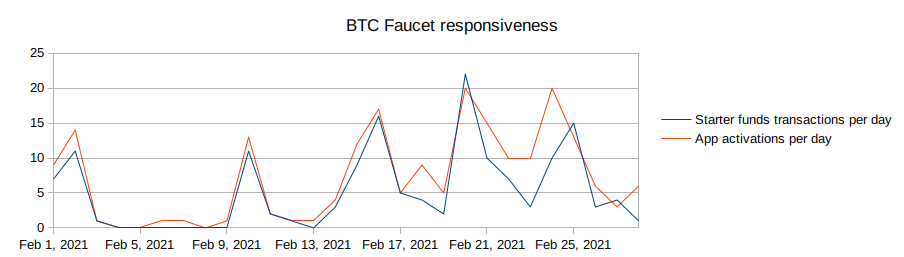
\includegraphics[width=1\textwidth]{evaluation/faucet-app-installs-3.png}
    \caption{Graph showing the relationship between faucet transactions of 10BTC and app activations}
    \label{fig:faucet-app-installs}
\end{figure}

\subsection{Flow of money to artists}
The datasets used to create the plots shown in figs. \ref{fig:artist-income} and \ref{fig:transactions} are received by scraping blockchain block data from our Bitcoin node. Fig. \ref{fig:artist-income} shows the relation between created blocks and money transacted per block (cumulative).

\begin{figure}
    \centering
    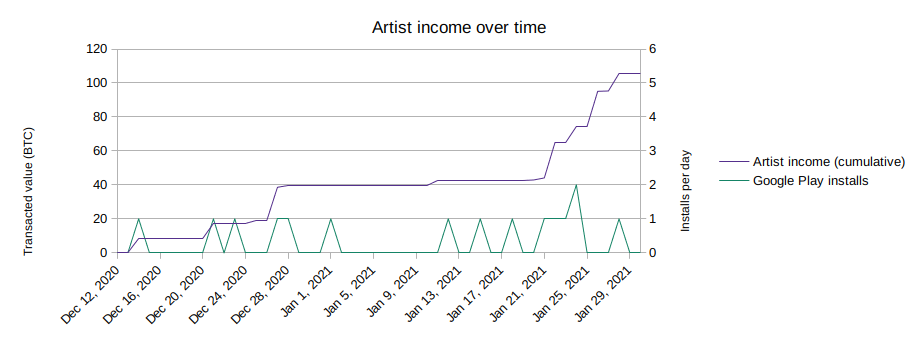
\includegraphics[width=1\textwidth]{evaluation/artist-income-3.png}
    \caption{Artist income (cumulative) versus app installations via the Google Play store, over time}
    \label{fig:artist-income}
\end{figure}
During initial experimentation, a small group of 10 people installed MusicDAO, with the task to stream music and spend their starter budget (10 coins) on donations to artists.

In regards of the timing of events, we expect to see most transaction activities to happen shortly after app installation. A correlation of these two events can be seen in the time intervals Dec. 14 - Dec. 28 and from Jan. 20 onwards.

We observe that the \textit{total artist income} (all received coins through donations from users) is $T=105.3$ coins over a time-span of 48 days. During this time-frame, there were at least 15 unique app installations through the Google Play console, which means that these users were given a combined budget $B\geq 150$. As the amount of installations is higher than the amount of users, some users may have installed the application on more than one device. $T\leq B$ conforms the validity of the artist income measurement and shows the effectiveness of the decentralized financial infrastructure in a small network of users.

\subsection{Block creation and transactions}
\begin{figure}
    \centering
    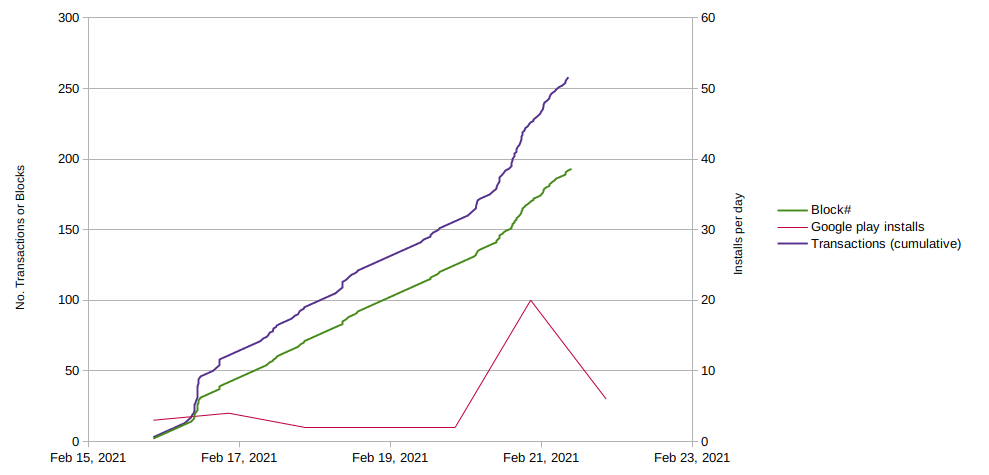
\includegraphics[width=0.9\textwidth]{evaluation/transactions-torrentfreak-3.png}
    \caption{Transactions (cumulative) over time and block creation (1 hour block interval)}
    \label{fig:transactions}
\end{figure}
During a 7-day public trial, we configured the Bitcoin node with a block interval of 1 hour. This block creation interval is well adopted by the node, as a steady linear growth can be seen in fig. \ref{fig:transactions}. This graph also shows the effect of an influx of users: On 20 Feb 2021, MusicDAO was promoted in a news article\footnote{\url{https://torrentfreak.com/university-runs-massive-bittorrent-seedbox-to-showcase-music-streaming-app-210220/}}) leading to a 220\%+ growth in app installations on a weekly basis. This can be seen as \textit{Google Play installs} in fig. \ref{fig:transactions}. In the few days after this moment, the average transactions per block was significantly higher.

Note that the Bitcoin blockchain only contains timestamps for blocks, and no timestamps for individual transactions. This means we could not analyze transaction confirmation time in our uncontrolled experiment, as this requires the timestamp of creating a transaction. However, prediction and analysis of confirmation times in larger Bitcoin networks have already been performed multiple times in recent literature~\citep{kawase2017transaction}~\citep{koops2018predicting}.

\section{Controlled experiments}
During several controlled experiments, we were in control of a network of 10 Android devices, of which 5 virtual emulators and 5 real world devices. By performing several experiments, throughput and latency of several actions in this network is analyzed. Performing measurements in different network sizes (2 up to 10 devices), enables making predictions of the scalability of MusicDAO. Please note that the throughput 

\subsection{Downloading and streaming}
In order to analyze the effectiveness of a fully decentralized peer-to-peer network, we measure latency of events in two scenarios: (1) a network of phones and one central server, and (2) with only phones. The central server hosts a BitTorrent tracker and 50 releases (3.9GB in total). The tracker helps peers find active uploaders for the file they are interested in. In the peer-to-peer scenario, music data transfers are purely phone-to-phone, using BitTorrent DHT. \ref{fig:download-times} shows the download time of each stage in the downloading process. By measuring 10 runs per network configuration, we inspect the effects of a BitTorrent tracker and central server on throughput and handshake times.

The 4 different download stages marked in this figure are as follows.

\begin{enumerate}
    \item Time to receive metadata (including establishing handshake)
    \item Time to fill stream buffer
    \item Time to download first track
    \item Time to download full album
\end{enumerate}

\begin{figure}
    \centering
    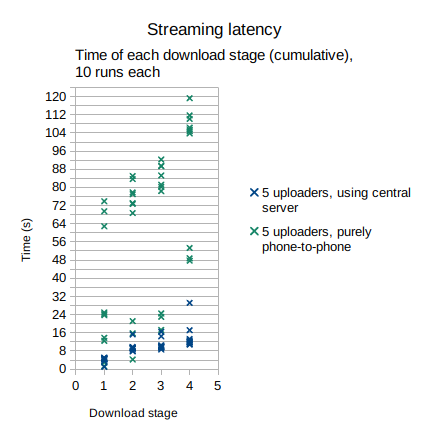
\includegraphics[width=0.5\textwidth]{evaluation/download-times-2.png}
    \caption{Average time spent per download stage. Measured by 20 runs in total, in two different network configurations.}
    \label{fig:download-times}
\end{figure}

The measurements show that a BitTorrent tracker significantly reduces transfer times, for a small BitTorrent swarm with 5 seeders. The largest difference is in the \textit{fetching metadata} stage, during which the device under test must find and connect with seeders. Discovering seeders over DHT requires asking multiple peers, and as such requires more time and messages before the download can start. Once the download starts, the runs using a tracker also reach significantly higher throughput, as the tracker assists the device in finding more seeders and healthier seeders. We found that the major factor slowing down download stages when using DHT only is the NAT puncturing stage, where devices try to connect to each other when there are one or more NAT devices in between. As expected, finding peers over DHT is also slower than via a tracker, however the time taken to create a handshake during NAT puncturing has a much larger effect on the peer-to-peer connecting time (the time taken to create a reliable connection for data transfer). 

In order to analyze the robustness of data transfers in the network, we measure the download speed over time after a successful handshake has been performed. \ref{fig:download-traces} shows 5 traces of downloading a 38 Megabyte album. The red line shows the moving average over these 5 runs. The slow-start nature of BitTorrent can be observed here. Roughly the first 5 seconds are used for fetching the BitTorrent metadata (see also \ref{fig:download-times}). 

\begin{figure}
    \centering
    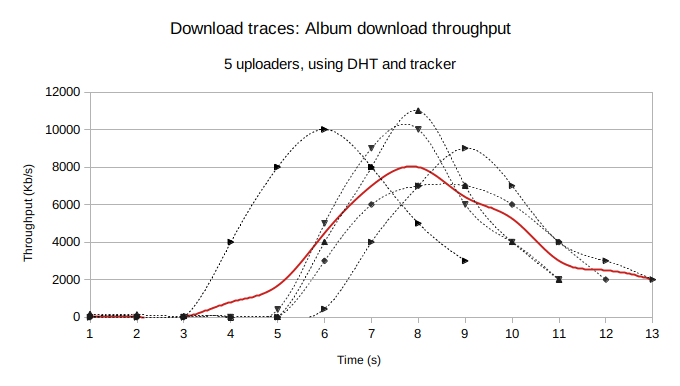
\includegraphics[width=0.8\textwidth]{evaluation/download-traces.png}
    \caption{5 traces of download throughput, downloading an album of around 38 Mbs. Measured with Nokia 7.}
    \label{fig:download-traces}
\end{figure}

Note that all devices evaluated in experiments \ref{fig:download-times} and \ref{fig:download-traces} use Bittorrent Local Peer Discovery. This means that some of the data transfers may be over local area network, which reaches considerably higher throughput than regular transfers over TCP across NATs.

The implemented streaming algorithm uses the BitTorrent priorities system. The first $x=5$ pieces at the selected portion of the file (by default, the start of the file) have a higher priority than the other pieces. However, even though some pieces $A$ have higher priority than other pieces $B$, BitTorrent does not guarantee that all $a\in A$ are received earlier before any $b\in B$. Therefore, the actual ordering of the received pieces is non-deterministic. The simple heuristic used in the streaming algorithm is: start playing the file when 30\% has been downloaded; but this does not always work and this leads to inconsistent stream buffer times. Additionally, we use the assumption that the header of the audio file is at the first few bytes of the file, but this is not always true.

There is ongoing research related to peer-to-peer streaming in literature that can be used to improve our streaming algorithm~\citep{erman2008piece}~\citep{akkanen2017continuous}.

\subsection{Content discovery}
Fig. \ref{fig:content-discovery} shows measurements of an Android device discovering content, after running MusicDAO for the first time. More specifically, it is a measurement of music metadata, received as TrustChain blocks. All participating devices are configured as follows: Every device sends a random block to a random peer every 5 seconds. A Nokia 7 Android device ran the MusicDAO in an idle state for 5 minutes. The app measured the amount of content metadata discovered every 2 seconds. 

\subsubsection{\textbf{Mathematical model}}
For evaluating content discovery over time, we compare three different experiments with a mathematical model for expected discovered items over time.

\begin{itemize}
    \item Gossip interval $t=5$ seconds
    \item Total items to discover: $R=50$
\end{itemize}

Every time interval, all devices send one music block to a random neighbor. As such, the expected amount of blocks received in one interval is 1. When receiving a music block, the chance that it is a block that has not been received before is $$\frac{R-r}{R}$$ with $r\leq R$ the amount of items received so far. It follows that the expected value for the cumulative amount of unique items discovered after $x$ iterations is $$E[R]=R(1-(\frac{R-1}{R})^{x})$$ where $$x=\frac{1}{t}$$ This expected value $E[R]$ over time is plotted in \ref{fig:content-discovery} as Model.

As every device sends one item per time interval to a neighbor, the gossiped items per time interval is equal to network size $n$. This means message complexity $M$ is equal to network size: $$M=O(n)$$

Every device participating in gossiping sends 1 message and receives, on average, 1 message back. So the expected messages to process is $E[M]=2$ per iteration. Therefore the message complexity for a single device is $$M=O(1)$$ This means that the network size does not affect the message processing workload of each device, and makes the algorithm highly scalable.

\begin{figure}
    \centering
    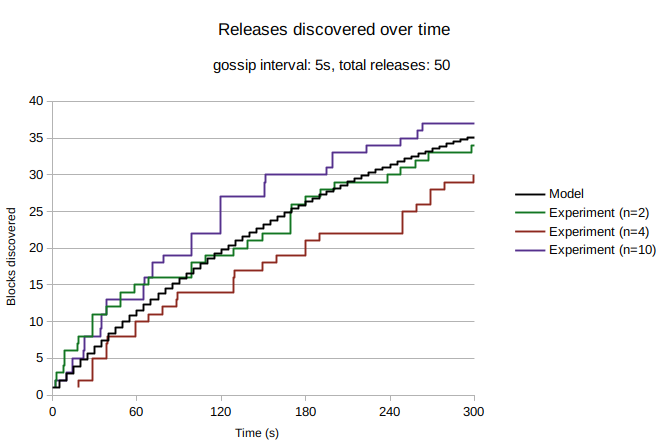
\includegraphics[width=0.8\textwidth]{evaluation/expected-vs-simulated-releases-2.png}
    \caption{Measurements of content discovery: releases discovered after a fresh installation. $n$: network size (amount of Android devices)}
    \label{fig:content-discovery}
\end{figure}

In \ref{fig:content-discovery} we can see a correlation between model and experiment for all network sizes $n=2$, $n=4$ and $n=10$. In these results, we can roughly observe logarithmic growth, as expected in the mathematical model. It must be noted that only one run of 5 minutes per network size was performed. More experimentation with larger network sizes should be done, to make further conclusions of scalability of the content discovery algorithm and its implementation.

\subsection{Random access latency}
Random access latency of metadata is evaluated through measuring search latency. Search latency is the round-trip time between initiating keyword search and receiving metadata for the release. During this experiment, the content that was searched for was present in all devices except the one under test. The distributed search algorithm (alg. \ref{alg:algorithm-distributed-search}) is used with the following parameters.

\begin{itemize}
    \item $maxPeers=20$
    \item $ttl=1$ 
\end{itemize}

This means that a maximum of 20 neighbors are contacted when performing a search, and that search is not recursive; meaning only neighbors are contacted (not neighbors of neighbors). We expect that random access latency does not increase in correspondence to relation to its network size.

For three different network sizes of 2, 6 and 10, 10 runs are done and the latency and average latency are plotted in \ref{fig:search-latency}. We observe that for these 20 runs, latency is $<1s$. Another observation is: increase in network size (10 versus 2) does not negatively affect latency. Current music streaming systems have a search latency of roughly $<2s$ in ideal situations.

% Re-do this experiment with a very fast GUI latency
\begin{figure}
    \centering
    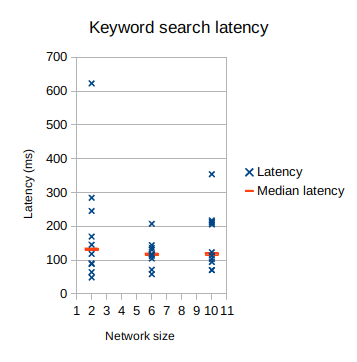
\includegraphics[width=0.5\textwidth]{evaluation/search-latency-2.png}
    \caption{Search latency of performing keyword search}
    \label{fig:search-latency}
\end{figure}

It should be noted that message complexity of the search algorithm grows exponentially with the value of \textit{time-to-live} (ttl). For time-to-live $T$ and the maximum number of neighboring peers to ask $P$, the amount of messages for a single search is $p^T$ for $p\leq P$. This leaves a message complexity of $O(P^T)$. This could be improved by using a different distributed data structure that is optimized for search, such as a balance tree or a distributed hash table. 

\section{Device connectivity and network bootstrapping}
During experimentation, some of the Bittorrent traffic on Android devices were blocked by Network Address  Translators (NATs). MP3 transfers over Bittorrent were slowed down by this. The NAT Port Mapping Protocol (NAT-PMP) was used to be able to establish connections between different devices. NAT-PMP establishes connections using port scanning and port forwarding. However, this is a lengthy process: we observed that establishing such a connection usually takes more than 2 minutes. Analyzing and improving this process should be investigated in future distributed systems research.

Our goal, as described in the Design section, was to create a phone-only network. This is not fully accomplished as we use a bootstrap node to tackle the \textit{peer-to-peer bootstrap problem}. As recognized by \cite{wolinsky2010addressing}, the peer-to-peer bootstrap problem is the problem of finding peers in a P2P overlay network, when there are no connected peers to begin with. This is a widely known, yet unsolved problem for any peer-to-peer network, and it is also relevant in MusicDAO. 

It must be noted that a bootstrap node is not necessary when you can connect to a peer that is already on the MusicDAO network, for example via a local area network or Bluetooth. Moreover, a bootstrap node can be discarded once the bootstrapping procedure is successful.

\section{Scalability}
We presented an infrastructureless network of phones that together form a fully operating application. During controlled experiments, a network size of up to 10 phones was used. Now we present our expectations of scalability beyond 10 active devices. 

As every device cooperates in the network by being both an uploader and downloader for content, the network size should not affect download speeds for users. The bandwidth, processing power and storage capacity of the application should naturally grow with the amount of users. An important note is that we do not take into account free-riders (peers that use the network but do not deliver resources) or adversaries (peers that perform attacks such as network flooding or sybil attack).

The system is scalable by using a scalable accounting system (see \ref{sec:distributed-storage}) and distributed file system (see \ref{sec:p2p-music-sharing}). Every device records its own history. When a device wants to publish music, it only transacts with one other party, to sign the metadata record. As such, there is no global consensus, nor a global ordering of transactions, so all records are processed in parallel. In addition, by using BitTorrent as the streaming/content layer, any participant can publish a torrent with music, without needing to interact with any other peer (in contrary to centralized streaming infrastructure and to IPFS). 

The transaction system, Bitcoin, may become a bottleneck in scalability~\citep{chauhan2018blockchain}. It has a single, global blockchain and blocks take on average 10 minutes to mine. There are other, more scalable protocols for transacting cryptocurrency in active development~\citep{lemahieu2018nano}, but they are not yet mature. However, our financial system of wallets using public-key cryptography is easily adaptable to any other cryptocurrency. We do not consider centralized technologies as that would concentrate power, in contrary to the aim of this thesis.

\section{Infrastructure cost}
% Proof-of-stake protocols for cryptocurrencies can result in lower transaction fees
The experimental environment made use of a bitcoin miner, running on a dedicated server continuously throughout the experimentation phase. At least one miner is necessary on our test network in order to process payments. The use of a dedicated server contradicts our design of a zero-server software system, and creates a single point of failure. However, this situation can be improved by decentralizing the network: by running miners on each device participating in the network, the resources become more balanced, and this would reduce the risk of hardware failures.

We use Bitcoin as peer-to-peer electronic cash system. Bitcoin uses transaction fees for every transaction. In our uncontrolled experiments with MusicDAO, we observed transaction fees of $<0.1‰$ coins. More specifically, the average transaction fee was $3.778\cdot10^{-4}$ coins. As such we cannot say that artists receive 100\% of the donation money from users. Although this number is low in our experiments, this fee is calculated dynamically and can grow larger under other network conditions, as shown in recent empirical research~\citep{moser2015trends}. 

On the other hand, the Bitcoin transaction fee is not a roadblock for building the Robot Economy in software, as our presented framework makes no statements on the type of currency used. For example, in MusicDAO, Bitcoin can be trivially swapped for any other currency as long as that currency uses a digital peer-to-peer public key infrastructure with public wallet addresses. As such, a different crypto-currency with lower transaction fees (such as Nano~\citep{lemahieu2018nano}) can be used.

\section{Battery usage}
% Add image from Matt Skala?
Any fully decentralized, peer-to-peer mobile app should continuously communicate with peers, also when the app is not in the foreground, in order to optimally contribute to the health of the network. To do this, TrustChain Superapp sends regular keep-alive messages in order to track the status of peers. The Superapp runs in the background as an Android service, so it still sends keep-alive messages when the app is out of focus. The downside is that this appears to have a major effect on battery usage, as found in previous experimentation by \cite{mattskala2020}. The author found that, during a 10 hour experiment, when a Google Pixel phone runs the app in the background and is connected to 20 peers, its battery consumption is roughly 10 times higher than normally.

The stress of MusicDAO on battery usage could be reduced by adjusting the peer-to-peer connectivity protocol of IPv8, such as by reducing the interval of keepalive messages. This requires further investigation and more research.